\begin{figure}[H]
    \begin{center}
        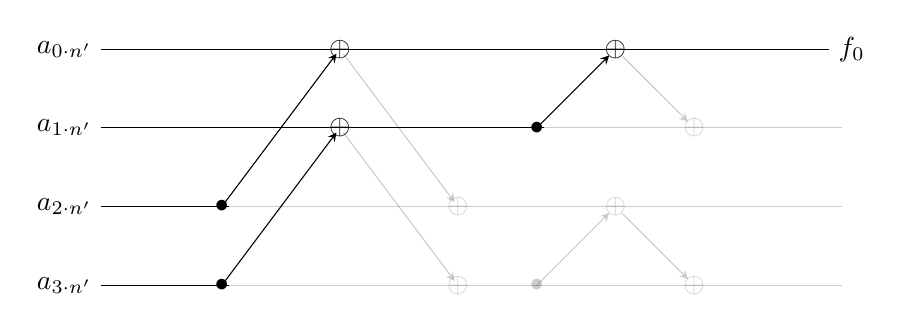
\begin{tikzpicture}
            \node (in4) at (0,3) {$a_{0\cdot n^\prime}$};
            \node (in3) at (0,2) {$a_{1\cdot n^\prime}$};
            \node (in2) at (0,1) {$a_{2\cdot n^\prime}$};
            \node (in1) at (0,0) {$a_{3\cdot n^\prime}$};
            \node (truncout4) at (10,3) {$f_0$};
            \node (truncout3) at (6,2) {};
            \node (truncout2) at (2,1) {};
            \node (truncout1) at (2,0) {};
            \node (out3) at (10,2) {};
            \node (out2) at (10,1) {};
            \node (out1) at (10,0) {};


            \node(m1) at (2, 0) {$\bullet$};
            \node(m2) at (2, 1) {$\bullet$};
            \node(m3) at (6, 2) {$\bullet$};
            \node[opacity=0.2](m4) at (6, 0) {$\bullet$};
            \node[opacity=0.2](a1) at (5, 0) {$\oplus$};
            \node[opacity=0.2](a2) at (5, 1) {$\oplus$};
            \node[opacity=0.2](a3) at (8, 2) {$\oplus$};
            \node[opacity=0.2](a4) at (8, 0) {$\oplus$};
            \node(b1) at (3.5, 2) {$\oplus$};
            \node(b2) at (3.5, 3) {$\oplus$};;
            \node(b3) at (7, 3) {$\oplus$};
            \node(b4)[opacity=0.2] at (7, 1) {$\oplus$};

            

            \draw[-, shorten >=-6pt] (in1) -- (truncout1);
            \draw[-, shorten >=-6pt] (in2) -- (truncout2);
            \draw[-, shorten >=-6pt] (in3) -- (truncout3);
            \draw[-, opacity=0.2, shorten <=-6pt] (truncout1) -- (out1);
            \draw[-, opacity=0.2, shorten <=-6pt] (truncout2) -- (out2);
            \draw[-, opacity=0.2, shorten <=-6pt] (truncout3) -- (out3);
            \draw[-] (in4) -- (truncout4);

            \draw[-stealth, shorten >=-6.5pt] (m1.center) -- (b1);
            \draw[-stealth, shorten >=-6.5pt, shorten <=-6.5pt, opacity=0.2] (b1) -- (a1);
            \draw[-stealth, shorten >=-6.5pt] (m2.center) -- (b2);
            \draw[-stealth, shorten >=-6.5pt, shorten <=-6.5pt, opacity=0.2] (b2) -- (a2);
            \draw[-stealth, shorten >=-6.5pt] (m3.center) -- (b3);
            \draw[-stealth, shorten >=-6.5pt, shorten <=-6.5pt, opacity=0.2] (b3) -- (a3);
            \draw[-stealth, shorten >=-6.5pt, opacity=0.2] (m4.center) -- (b4);
            \draw[-stealth, shorten >=-6.5pt, shorten <=-6.5pt, opacity=0.2] (b4) -- (a4);


        \end{tikzpicture}
    \end{center}
    \caption{A 2-layer Truncated FFT}
    \label{fig:trunc-fft} 
\end{figure}